\newcommand{\OPT}[1]{\texttt{#1}}
\newcommand{\OPTprintValidExecutionTraces}{-\,-print-Execution-Traces}
\newcommand{\OPTprintInvalidExecutionTraces}{-\,-print-invalid-Execution-Traces}
\newcommand{\OPTprintMessageTraces}{-\,-print-Message-Traces}
\newcommand{\OPTprintDeploymentEquivalenceClasses}{-\,-print-Deployment-Equivalence-Classes}
\newcommand{\OPTprintAssemblyEquivalenceClasses}{-\,-print-Assembly-Equivalence-Classes}
\newcommand{\OPTplotDeploymentSequenceDiagrams}{-\,-plot-Deployment-Sequence-Diagrams}
\newcommand{\OPTplotAssemblySequenceDiagrams}{-\,-plot-Assembly-Sequence-Diagrams}
\newcommand{\OPTplotCallTrees}{-\,-plotCallTrees}
\newcommand{\OPTplotAggregatedDeploymentCallTree}{-\,-plot-Aggregated-Deployment-Call-Tree}
\newcommand{\OPTplotAggregatedAssemblyCallTree}{-\,-plot-Aggregated-Assembly-Call-Tree}

\newcommand{\OPTplotContainerDependencyGraph}{-\,-plot-Container-Dependency-Graph}
\newcommand{\OPTplotDeploymentComponentDependencyGraph}{-\,-plot-Deployment-Component-Dependency-Graph}
\newcommand{\OPTplotAssemblyComponentDependencyGraph}{-\,-plot-Assembly-Component-Dependency-Graph}
\newcommand{\OPTplotDeploymentOperationDependencyGraph}{-\,-plot-Deployment-Operation-Dependency-Graph}
\newcommand{\OPTplotAssemblyOperationDependencyGraph}{-\,-plot-Assembly-Operation-Dependency-Graph}

The examples presented in this section were generated based on the %
monitoring data which can be found in the directory %
\dir{\distributedTestdataDirDistro/}. It consists of 1635 traces %
of the Bookstore application with AspectJ-based instrumentation, %
as described in Section~\ref{sec:traceAnalysis:instr:AspectJ}. %
In order to illustrate the visualization of distributed traces, %
the hostname of the \class{Catalog}'s method \method{getBook} was %
probabilistically changed to a second hostname. %
For a more detailed description on the underlying formalisms, %
we refer to our technical report~\cite{vanHoornRohrHasselbringWallerEhlersFreyKieselhorst2009TRContinuousMonitoringOfSoftwareServicesDesignAndApplicationOfTheKiekerFramework}.

\subsection{Textual Trace and Equivalence Class Representations}

\subsubsection{Execution Traces}\label{sec:example:executionTraces}%

Textual execution trace representations of valid/invalid traces are written to %
an output file using the command-line options \OPT{\OPTprintValidExecutionTraces} and %
\OPT{\OPTprintInvalidExecutionTraces}. %
Listing~\ref{lst:appendix:traceAnalysisExample:executionTraces} %
shows the execution trace representation for the valid trace \ldots6129.

\setTextListing
\lstinputlisting[firstline=1,lastline=5,escapechar={},%
caption=Textual output of trace 6488138950668976129's execution trace representation,%
label=lst:appendix:traceAnalysisExample:executionTraces]%
{images/example-plots/executionTraces.txt}

\subsubsection{Message Traces}\label{sec:example:messageTraces}%

Textual message trace representations of valid traces are written to an output %
file using the command-line option \OPT{\OPTprintMessageTraces}. %
Listing~\ref{lst:appendix:traceAnalysisExample:messageTraces} %
shows the message trace representation for the valid trace \ldots6129.

\setTextListing
\lstinputlisting[firstline=1,lastline=9,escapechar={},%
caption=Textual output of trace 6488138950668976129's message trace representation,%
label=lst:appendix:traceAnalysisExample:messageTraces]%
{images/example-plots/messageTraces.txt}

\subsubsection{Trace Equivalence Classes}\label{sec:example:traceEquivClasses}%

Deployment/assembly-level trace equivalence classes are computed and written %
to output files using the command-line options \OPT{\OPTprintDeploymentEquivalenceClasses} %
and \OPT{\OPTprintAssemblyEquivalenceClasses}. %
Listings~\ref{lst:appendix:traceAnalysisExample:traceDeploymentEquivClasses} and %
\ref{lst:appendix:traceAnalysisExample:traceAssemblyEquivClasses} show the %
output generated for the monitoring data used in this section. %

\setTextListing
\lstinputlisting[caption=Textual output of information on the \textit{deployment-level} trace equivalence classes,%
label=lst:appendix:traceAnalysisExample:traceDeploymentEquivClasses]
{images/example-plots/traceDeploymentEquivClasses.txt}

\setTextListing
\lstinputlisting[caption=Textual output of information on the \textit{assembly-level} trace equivalence class,%
label=lst:appendix:traceAnalysisExample:traceAssemblyEquivClasses]%
{images/example-plots/traceAssemblyEquivClasses.txt}

\pagebreak

\subsection{Sequence Diagrams}\label{sec:example:seqDiagrams}%

\subsubsection{Deployment-Level Sequence Diagrams}\label{sec:example:deploymentSeqDiagrams}%

Deployment-level sequence diagrams are generated using the command-line option \OPT{\OPTplotDeploymentSequenceDiagrams}. %
Figures~\ref{fig:appendix:traceAnalysisExample:SeqDiagrsDepl6129}--\ref{fig:appendix:traceAnalysisExample:SeqDiagrsDepl6141} %
show these sequence diagrams for each deployment-level %
trace equivalence representative (Section~\ref{sec:example:traceEquivClasses}).

\begin{figure}[h]\centering
\subfigure[Trace \ldots{}6129]{\label{fig:appendix:traceAnalysisExample:SeqDiagrsDepl6129}%
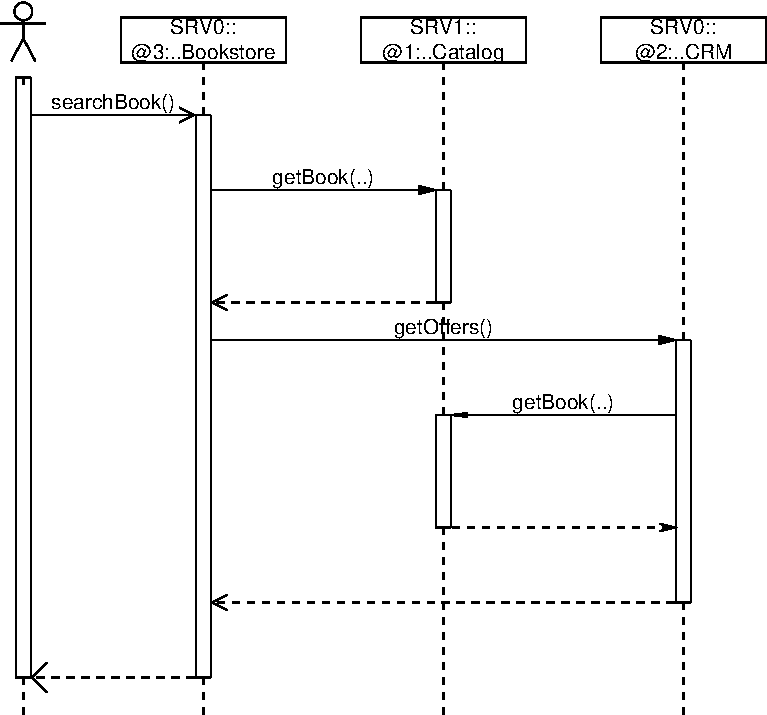
\includegraphics[scale=0.39]{images/example-plots/deploymentSequenceDiagram-6488138950668976129-crop}
}
\subfigure[Trace \ldots{}6130]{\label{fig:appendix:traceAnalysisExample:SeqDiagrsDepl6130}%
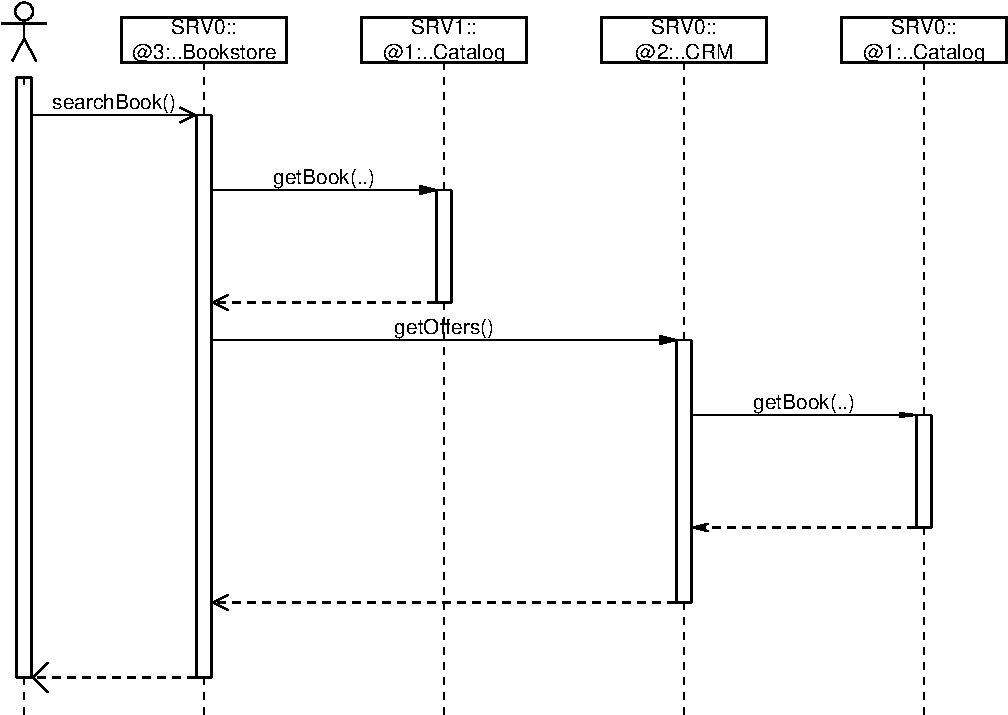
\includegraphics[scale=0.39]{images/example-plots/deploymentSequenceDiagram-6488138950668976130-crop}
}
\subfigure[Trace \ldots{}6131]{\label{fig:appendix:traceAnalysisExample:SeqDiagrsDepl6131}%
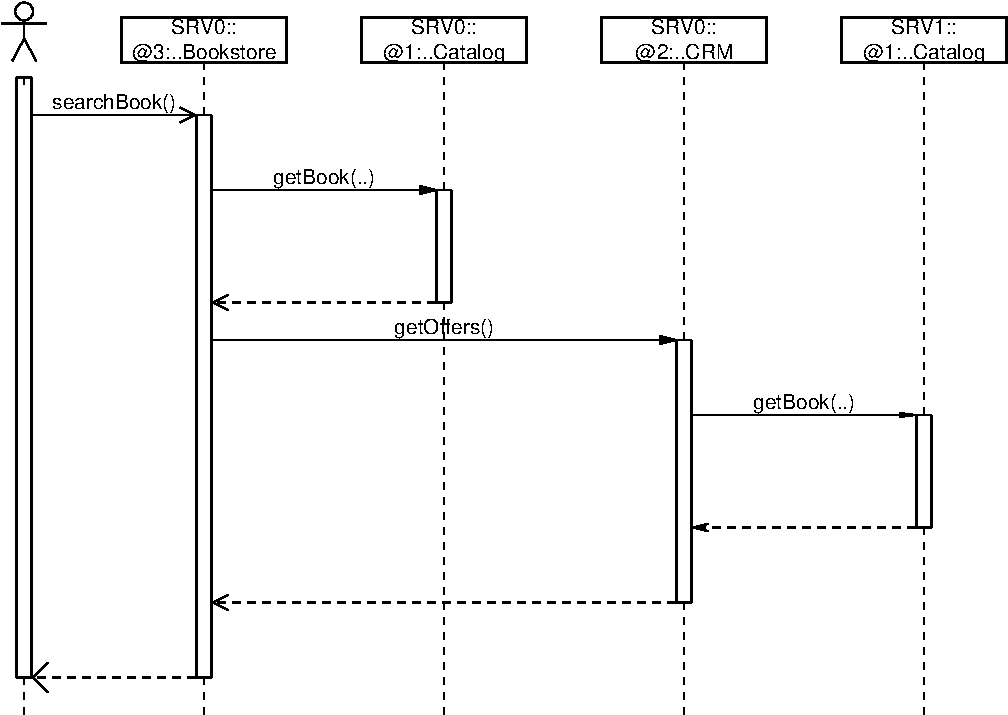
\includegraphics[scale=0.39]{images/example-plots/deploymentSequenceDiagram-6488138950668976131-crop}
}
\subfigure[Trace \ldots{}6141]{\label{fig:appendix:traceAnalysisExample:SeqDiagrsDepl6141}%
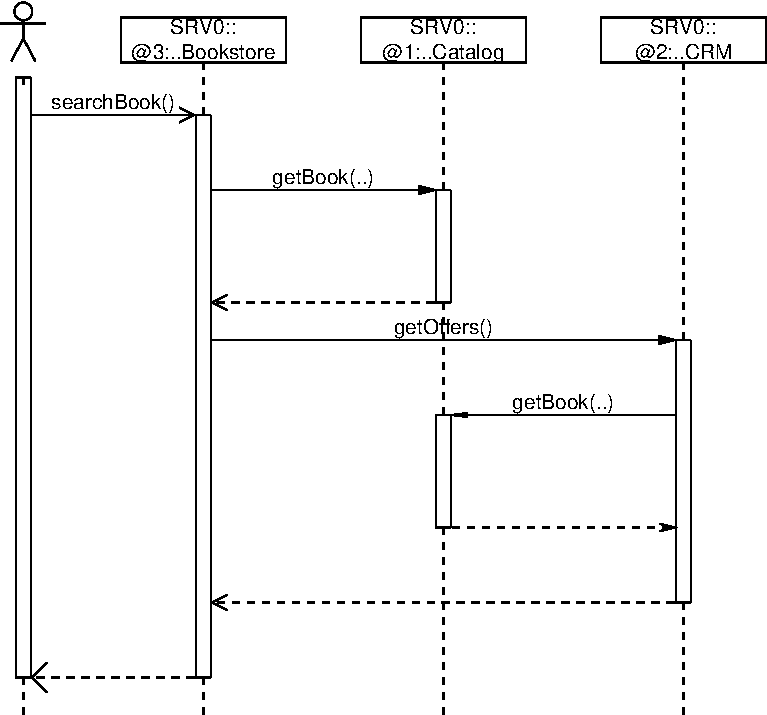
\includegraphics[scale=0.39]{images/example-plots/deploymentSequenceDiagram-6488138950668976141-crop}
}
\caption{\textit{Deployment-level} sequence diagrams of the trace %
equivalence class representatives (Listing~\ref{lst:appendix:traceAnalysisExample:traceAssemblyEquivClasses})}
\label{fig:appendix:traceAnalysisExample:SeqDiagrsDepl}
\end{figure}

\enlargethispage{2cm}

\subsubsection{Assembly-Level Sequence Diagrams}\label{sec:example:assemblySeqDiagrams}%

Assembly-level sequence diagrams are generated using the command-line option \OPT{\OPTplotAssemblySequenceDiagrams}. %
Figure~\ref{fig:appendix:traceAnalysisExample:SeqDiagrDepl6129} %
show the sequence diagram for the assembly-level trace equivalence representative %
(Section~\ref{sec:example:traceEquivClasses}).

\begin{figure}[h]\centering
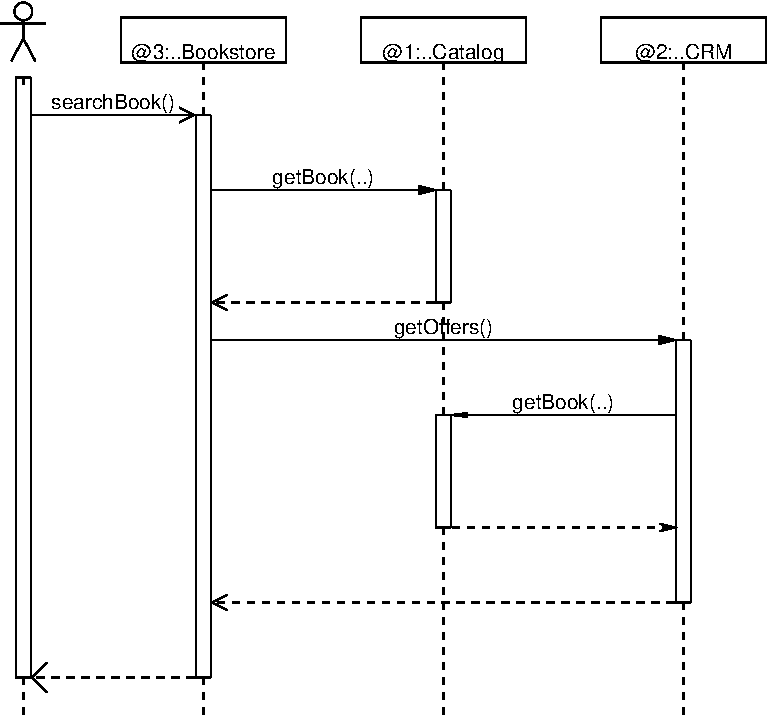
\includegraphics[scale=0.39]{images/example-plots/assemblySequenceDiagram-6488138950668976129-crop}
\caption{\textit{Assembly-level} sequence diagram of trace \ldots{}6129}
\label{fig:appendix:traceAnalysisExample:SeqDiagrDepl6129}
\end{figure}

\pagebreak

\subsection{Call Trees}\label{sec:example:callTrees}%

\subsubsection{Trace Call Trees}\label{sec:example:traceCallTrees}%

\enlargethispage{1.2cm}

Trace call trees are generated using the command-line option \OPT{\OPTplotCallTrees}. %
Figures~\ref{fig:appendix:traceAnalysisExample:TraceCallTrees6129}--\ref{fig:appendix:traceAnalysisExample:TraceCallTrees6141} %
show these call trees for each deployment-level %
trace equivalence representative (Section~\ref{sec:example:traceEquivClasses}).

\begin{figure}[h]\centering
\subfigure[Trace \ldots{}6129]{\label{fig:appendix:traceAnalysisExample:TraceCallTrees6129}%
\ \ 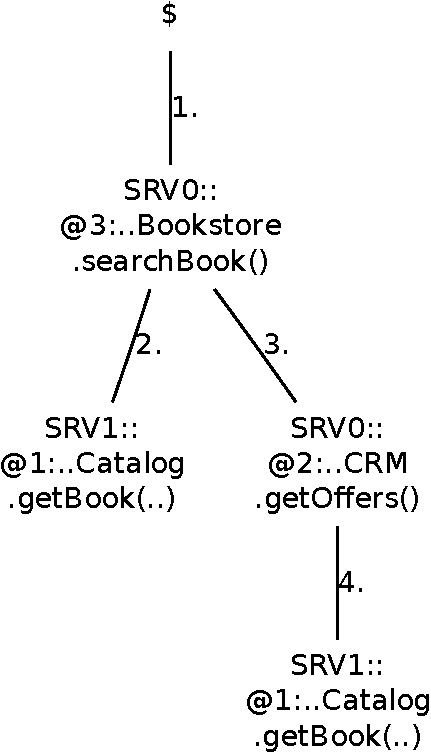
\includegraphics[scale=0.4]{images/example-plots/callTree-6488138950668976129-crop}\ \ 
}
\subfigure[Trace \ldots{}6130]{\label{fig:appendix:traceAnalysisExample:TraceCallTrees6130}%
\ \ 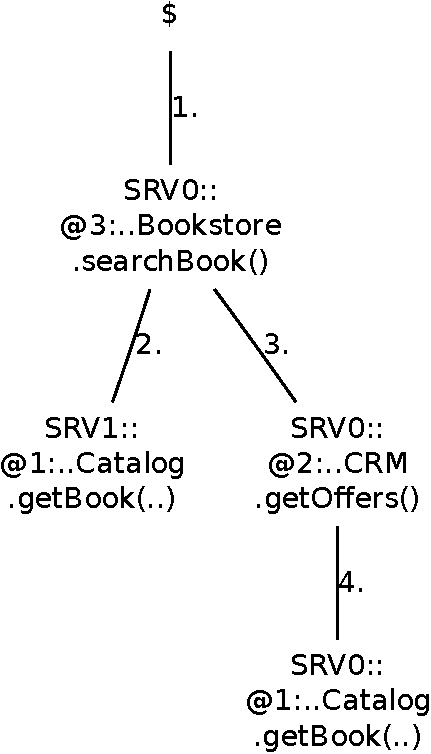
\includegraphics[scale=0.4]{images/example-plots/callTree-6488138950668976130-crop}\ \ 
}
\subfigure[Trace \ldots{}6131]{\label{fig:appendix:traceAnalysisExample:TraceCallTrees6131}%
\ \ 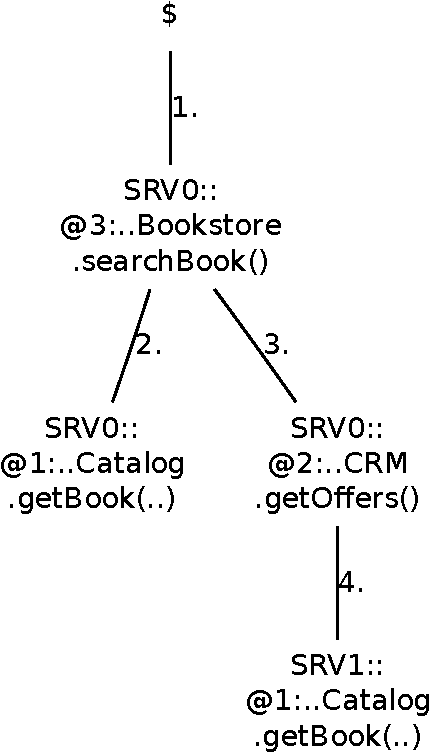
\includegraphics[scale=0.4]{images/example-plots/callTree-6488138950668976131-crop}\ \ 
}
\subfigure[Trace \ldots{}6141]{\label{fig:appendix:traceAnalysisExample:TraceCallTrees6141}%
\ \ 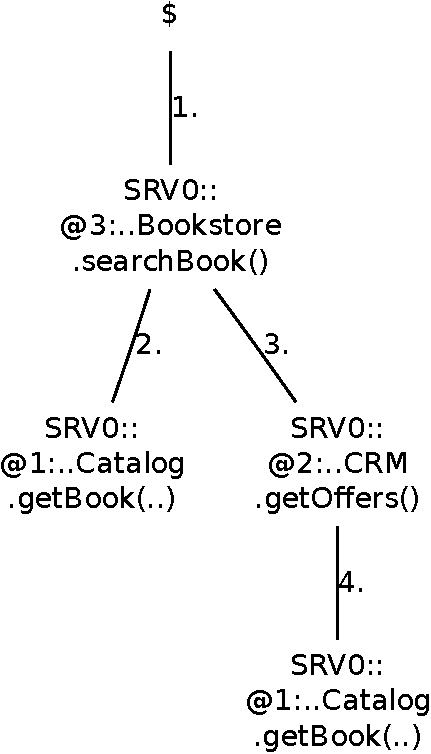
\includegraphics[scale=0.4]{images/example-plots/callTree-6488138950668976141-crop}\ \ 
}
\caption{Calls trees of the trace %
equivalence class representatives (Listing~\ref{lst:appendix:traceAnalysisExample:traceAssemblyEquivClasses})}
\label{fig:appendix:traceAnalysisExample:TraceCallTrees}
\end{figure}

% \newpage

\subsubsection{Aggregated Call Trees}\label{sec:example:aggregatedCallTrees}%

Aggregated deployment/assembly-level call trees are generated using the command-line options %
\OPT{\OPTplotAggregatedDeploymentCallTree} and \OPT{\OPTplotAggregatedAssemblyCallTree}. %
Figures~\ref{fig:appendix:traceAnalysisExample:AggregatedCallTreesDeployment} and \ref{fig:appendix:traceAnalysisExample:AggregatedCallTreesAssembly} %
show these aggregated call trees for the traces contained in the monitoring data %
used in this section. %

\begin{figure}[h]\centering
\subfigure[deployment-level]{\label{fig:appendix:traceAnalysisExample:AggregatedCallTreesDeployment}%
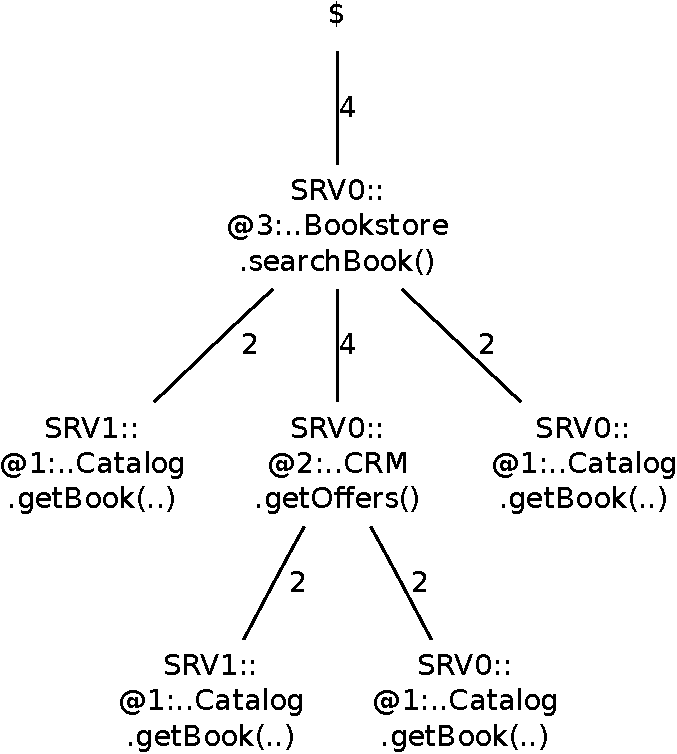
\includegraphics[scale=0.4]{images/example-plots/aggregatedDeploymentCallTree-crop}%
}
\subfigure[assembly-level]{\label{fig:appendix:traceAnalysisExample:AggregatedCallTreesAssembly}%
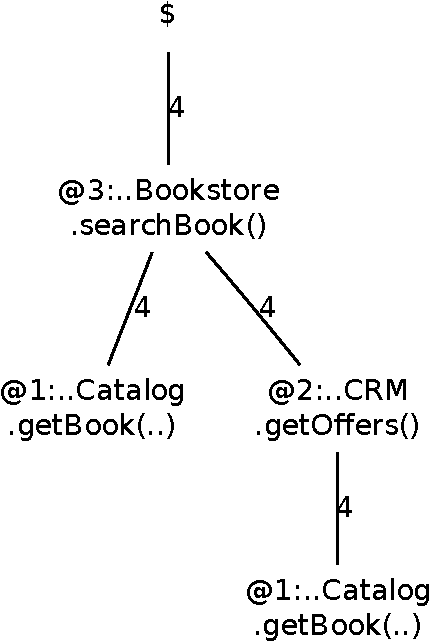
\includegraphics[scale=0.4]{images/example-plots/aggregatedAssemblyCallTree-crop}%
}
\caption{Aggregated call trees generated from the 1635~traces}
\label{fig:appendix:traceAnalysisExample:AggregatedCallTrees}
\end{figure}


\subsection{Dependency Graphs}

\subsubsection{Container Dependency Graphs}

A container dependency graph is generated using the command-line option %
\OPT{\OPTplotContainerDependencyGraph}. %
Figure~\ref{fig:appendix:traceAnalysisExample:ContainerDepGraph} shows the %
container dependency graph for the monitoring data used in this section. 

\begin{figure}[h]\centering
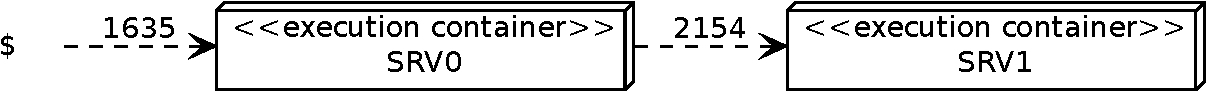
\includegraphics[scale=0.45]{images/example-plots/containerDependencyGraph-crop}
\caption{Container dependency graph}
\label{fig:appendix:traceAnalysisExample:ContainerDepGraph}
\end{figure}

\subsubsection{Component Dependency Graphs}

Deployment/assembly-level component dependency graphs are generated using the %
command-line options \OPT{\OPTplotDeploymentComponentDependencyGraph} and %
\OPT{\OPTplotAssemblyComponentDependencyGraph}. %
Figures~\ref{fig:appendix:traceAnalysisExample:ComponentDepGraphsDeployment} and %
\ref{fig:appendix:traceAnalysisExample:ComponentDepGraphsAssembly} show the %
component dependency graphs for the monitoring data used in this section. 

\begin{figure}[h]\centering
\subfigure[deployment-level]{\label{fig:appendix:traceAnalysisExample:ComponentDepGraphsDeployment}%
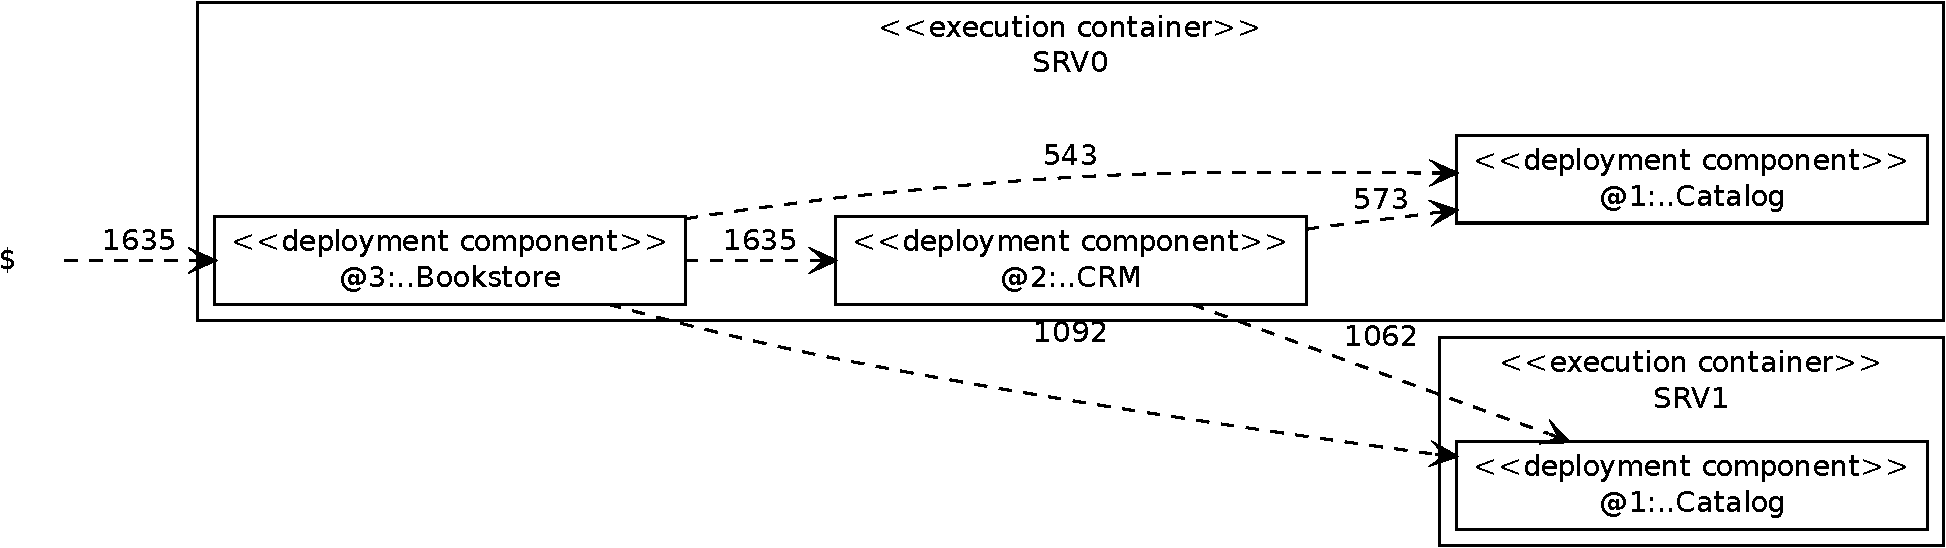
\includegraphics[scale=0.45]{images/example-plots/deploymentComponentDependencyGraph-crop}
}
\subfigure[assembly-level]{\label{fig:appendix:traceAnalysisExample:ComponentDepGraphsAssembly}%
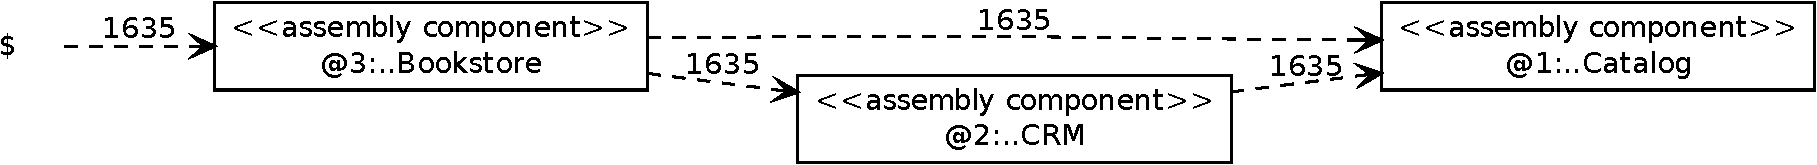
\includegraphics[scale=0.45]{images/example-plots/assemblyComponentDependencyGraph-crop}
}
\caption{Component dependency graphs}
\label{fig:appendix:traceAnalysisExample:ComponentDepGraphs}
\end{figure}

\subsubsection{Operation Dependency Graphs}

Deployment/assembly-level operation dependency graphs are generated using the %
command-line options \OPT{\OPTplotDeploymentOperationDependencyGraph} and %
\OPT{\OPTplotAssemblyOperationDependencyGraph}. %
Figures~\ref{fig:appendix:traceAnalysisExample:OperationDepGraphsDeployment} and %
\ref{fig:appendix:traceAnalysisExample:OperationDepGraphsAssembly} show the %
operation dependency graphs for the monitoring data used in this section. 

\begin{figure}[ht]\centering
\subfigure[deployment-level]{\label{fig:appendix:traceAnalysisExample:OperationDepGraphsDeployment}%
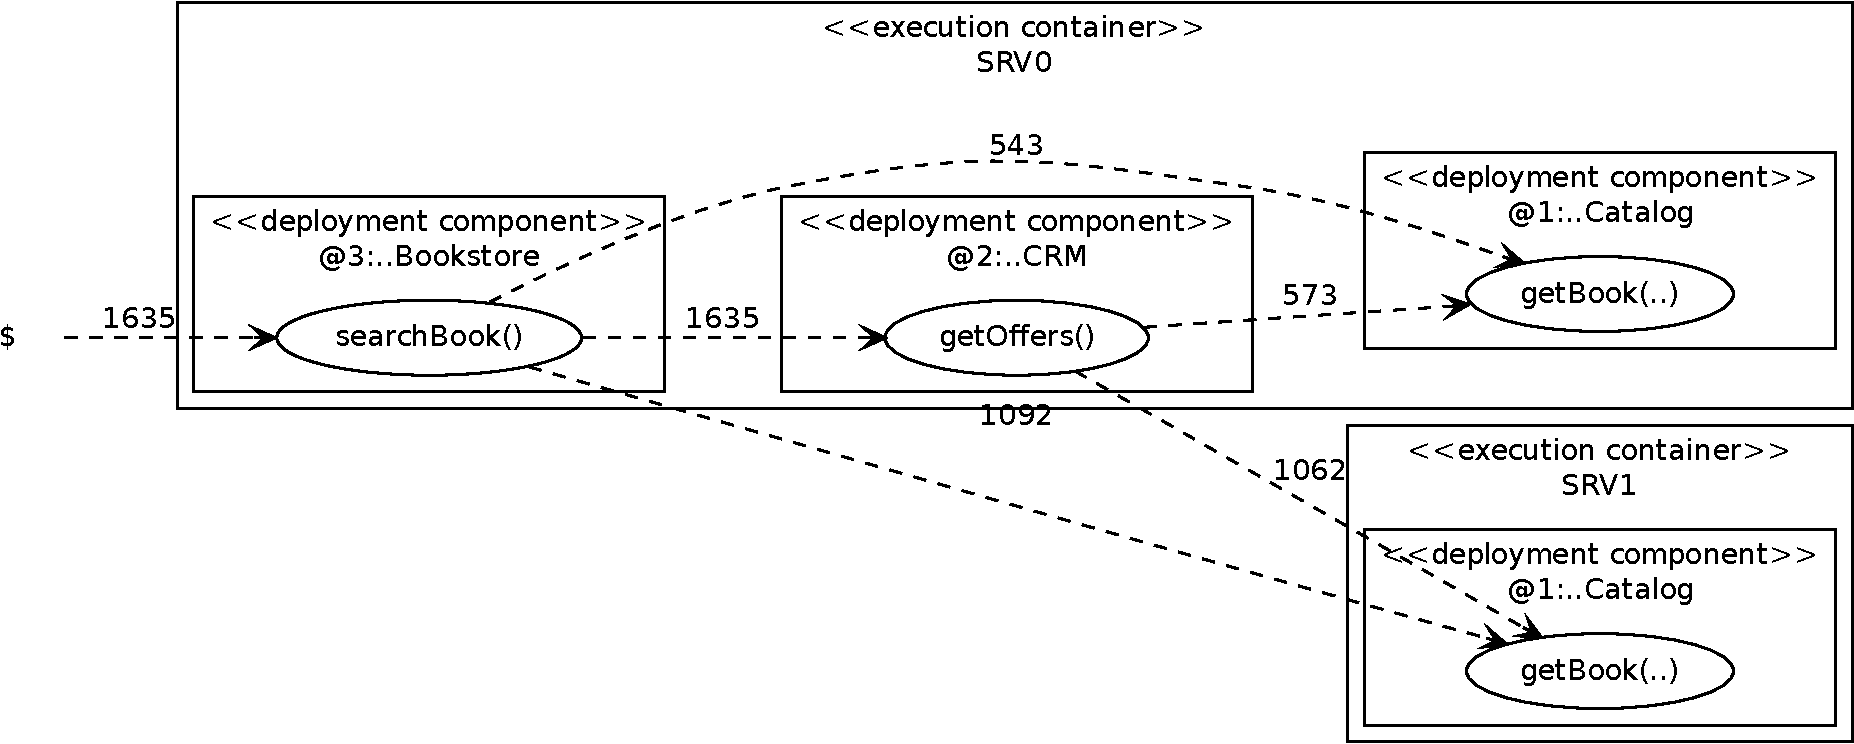
\includegraphics[scale=0.4]{images/example-plots/deploymentOperationDependencyGraph-crop}
}
\subfigure[assembly-level]{\label{fig:appendix:traceAnalysisExample:OperationDepGraphsAssembly}%
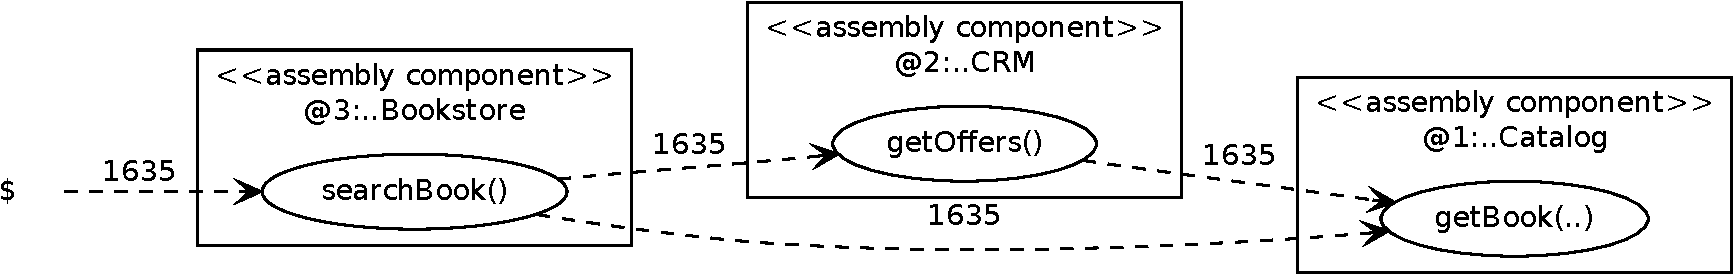
\includegraphics[scale=0.4]{images/example-plots/assemblyOperationDependencyGraph-crop}
}
\caption{Operation dependency graphs}
\label{fig:appendix:traceAnalysisExample:OperationDepGraphs}
\end{figure}

\subsection{HTML Output of the System Model}

\KiekerTraceAnalysis{} writes an HTML representation of the system model reconstructed %
from the trace data to a file \file{system-entities.html}. %
Figure~\ref{fig:appendix:traceAnalysisExample:htmlSystemModel} shows a screenshot %
of this file rendered by a web browser.

\pagebreak

\enlargethispage{3cm}

\begin{figure}[h]\centering
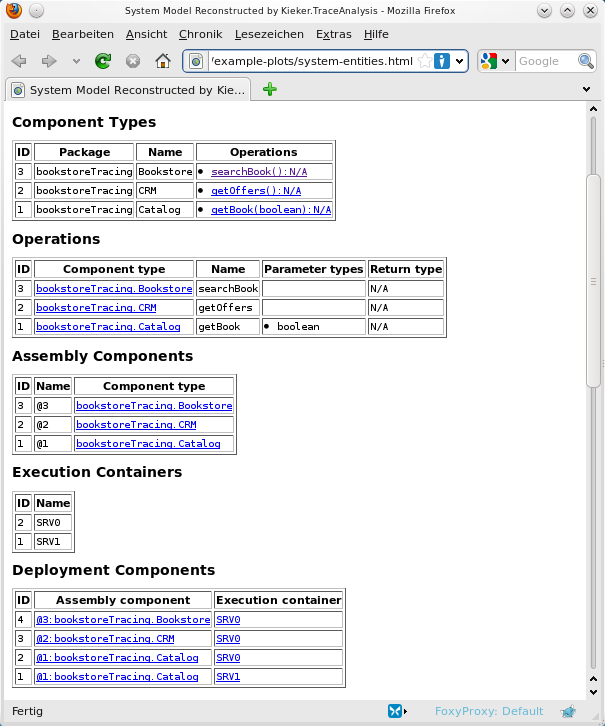
\includegraphics[width=0.5\textwidth]{images/example-plots/system-entities-html-FFscrsh.png}
\caption{HTML output of the system model reconstructed from the traces}
\label{fig:appendix:traceAnalysisExample:htmlSystemModel}
\end{figure}
